\section{Design of feedforward FXLMS system} \label{sec:systemDesign}
This appendix will go through the design of the system using a feedforward topology. The ANC system will be placed in a headphone with the microphones placed as seen on \autoref{fig:SystemHeadphone}. A B\&K TYPE 4128-C will be used as the HATS during tests. This means that the cancellation path will have a linear time-invariant (LTI) impulse response. 



\begin{figure}[H]
	\centering
	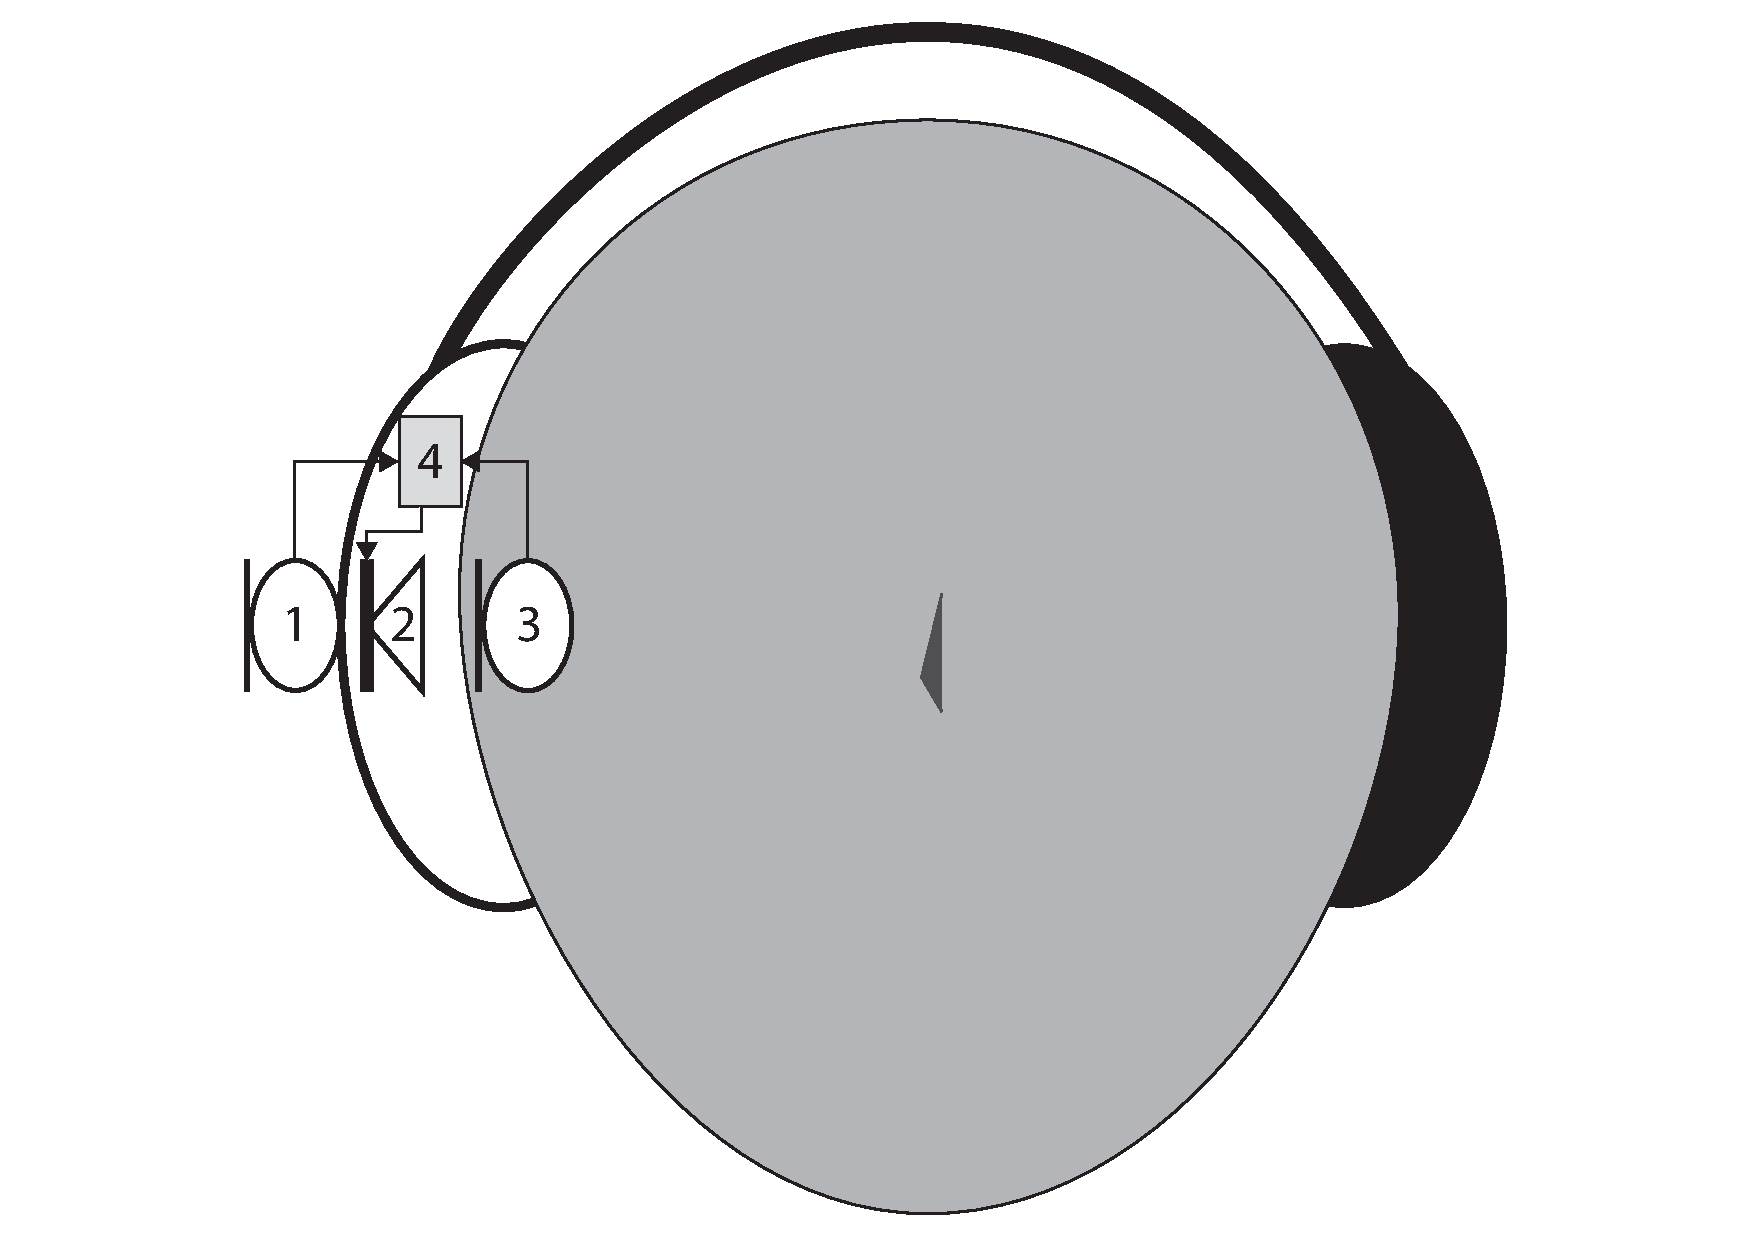
\includegraphics[width=0.8\textwidth]{Articleillustrations/SystemOverview}
	\caption{Illustration of the HATS wearing a headphone fitted with a ANC solution. Showing the reference microphone (1), a headphone loudspeaker (2), an error microphone (3) and a DSP (4).}
	\label{fig:SystemHeadphone}
\end{figure}  
%\todoKiis{I don't think we ever name 1,2,3 and 4 in the appendixes? DONE}

Because the cancellation path is LTI, the adaptive algorithm adjusting the cancellation path (CP) estimate will be omitted from the system. This means that the copy of the CP estimate will be a constant impulse response. The CP has been found as described in \autoref{sec:DT770CPjournal}. The used feedforward control system is shown in \autoref{fig:ANCFeedforwardAppendix} and is described in \autoref{sec:BasicSystem}.


\begin{figure}[H]
	\centering
	\tikzsetnextfilename{ANCFeedForwardAppendix}
	\resizebox{0.55\columnwidth}{!}{
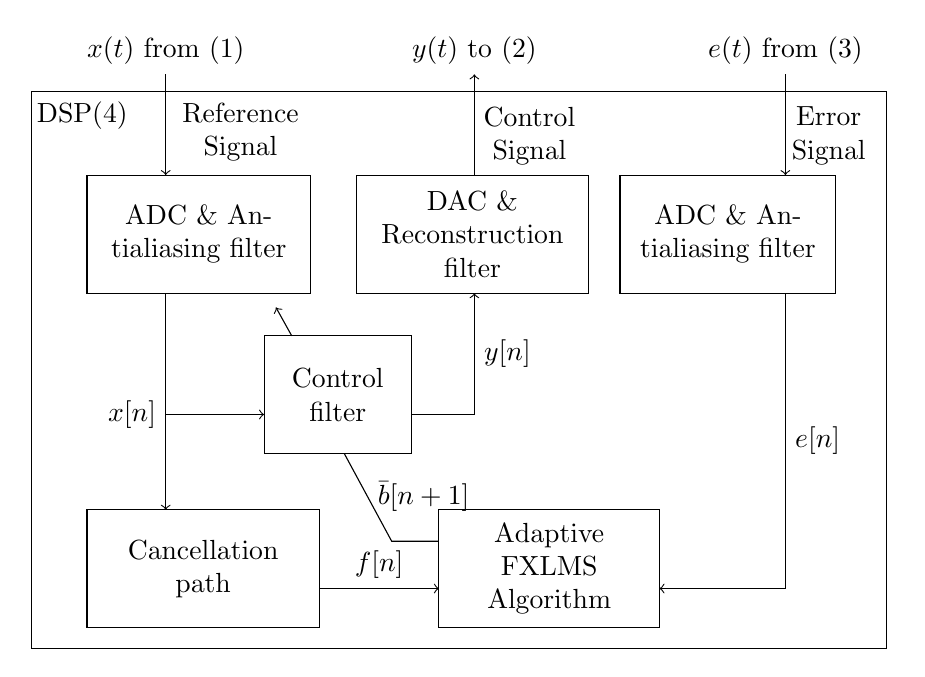
\begin{tikzpicture}
\draw  (-4,4.93) rectangle node[text width=2.5cm,align=center] {ADC \& Antialiasing filter} (-1.16,3.43);
\draw  (-4,0.68) rectangle node[text width=2.5cm,align=center] {Cancellation \\ path}(-1.05,-0.82);
\draw  (0.47,0.68) rectangle node[text width=2.5cm,align=center] {Adaptive FXLMS Algorithm} (3.27,-0.82);

\draw  (-1.75,2.89) rectangle node[text width=1.5cm,align=center,fill=white] {Control filter} (0.12,1.39);
\draw  (-0.58,4.93) rectangle node[text width=2.5cm,align=center] {DAC \& \\ Reconstruction filter}(2.37,3.43);
\draw  (2.77,4.93) rectangle node[text width=2.5cm,align=center] {ADC \& Antialiasing filter}(5.51,3.43);

\draw  (-4.71,5.99) rectangle (6.15,-1.08);
\node at (-4.06,5.69) {DSP(4)};
\node [text width=2cm,align=center] at (-2.05,5.48) {Reference Signal};

\draw[->] (-1.05,-0.32) -- node[above]{$f[n]$} (0.47,-0.32);

\draw[->] (4.87,3.43) -- node[right]{$e[n]$} (4.87,-0.32)  -- (3.27,-0.32);

\draw [->](4.87,6.21) node[above]{$e(t)$ from (3)} -- (4.87,4.93) ;
\draw [->](0.92,4.93)  --  (0.92,6.21) node[above]{$y(t)$ to (2)};
\draw [->](-3,3.43) -- (-3,0.68);

\draw [->](-3,1.89) node[left]{$x[n]$} -- (-1.75,1.89);

\draw[->] (0.12,1.89) -- (0.92,1.89) --node[right]{$y[n]$} (0.92,3.43);
\draw [->](-3,6.21) node[above]{$x(t)$ from (1)} -- (-3,4.93);
\node [text width=2cm,align=center] at (1.62,5.43) {Control Signal};
\node [text width=1.5cm,align=center] at (5.42,5.43) {Error Signal};

\draw (0.47,0.28) -- (-0.13,0.28) --node[above=0.25,right]{$\bar{b}[n+1]$} (-0.73,1.39);
\draw [->](-1.4,2.89) -- (-1.6,3.25);
\end{tikzpicture}}
	\caption{Block diagram of adaptive feedforward ANC system. Expansion of DSP (4) from \autoref{fig:SystemHeadphone}.}
	\label{fig:ANCFeedforwardAppendix}
\end{figure}



\subsection{FXLMS algorithm for FIR-filters}\label{subsec:fxlms}
The FXLMS is a gradient descent algorithm which iteratively changes the coefficients of the control filter by adding a calculated step to the current coefficients which should converge to a global minimum of the error criterion. The derivation of the FXLMS algorithm is given below. 
\begin{equation}\label{eq:FXLMSNewCoef}
\bar{b}(k+1) = \bar{b}(k) - \mu\nabla \bar{J}(k)
\end{equation}
Where:
\begin{description}
	\item[\text{$\nabla \bar{J}(k)$}] is the gradient of the error surface at the location given by the current weight coefficient.
	\item[\text{$\mu$}] is a convergence factor.
	\item[\text{$\bar{b}(k)$}] is the weight coefficients of the control filter written as  $\bar{b}(k)=[b_0(k),b_1(k) ,\dotsc, b_{L-1}(k)]^T$.
\end{description}
The error is defined as:
\begin{equation}\label{eq:FXLMSError}
e(k) = p(k) + s(k)
\end{equation}
Where:
\begin{description}
	\item[\text{$p(k)$}] is the primary noise source.
	\item[\text{$s(k)$}] is the counterphase signal.
\end{description}

The error criterion as a function of the filter weights is to be minimized, therefore the gradient of the error surface ($\nabla \bar{J}$) is calculated by differentiating the squared error, as shown in equation \ref{eq:FXLMSGradient}.
\begin{equation}\label{eq:FXLMSGradient}
\bar{J}(k) = e^2(k)
\end{equation}

Differentiating equation \ref{eq:FXLMSGradient} with respect to $b(k)$ yields equation \ref{eq:FXLMSGradientW(k)}. The last substitution can be made because $p(k)$ does not depend on $b(k)$. So the term $p(k)$ from equation \ref{eq:FXLMSError} does not influence the gradient of $e(k)$:

\begin{equation}\label{eq:FXLMSGradientW(k)}
\Delta \bar{b}(k) = \frac{\partial e^2(k)}{\partial \bar{b}(k)} = 2e(k)\frac{\partial e(k)}{\partial \bar{b}(k)} = 2e(k)\frac{\partial s(k)}{\partial \bar{b}(k)}
\end{equation}
$e(k)$ can be sampled. How to obtain s(k) is described below. \\
The controller output signal y(k) is given by equation \ref{eq:FXLMSOutput}.

\begin{equation}\label{eq:FXLMSOutput}
y(k) = \bar{b}^T(k)*\bar{x}(k) = \sum_{j=0}^{L-1} b_j(k)x(k-j)
\end{equation}
Where:
\begin{description}
	\item[\text{$\bar{x}(k)$}] = $[x(k) x(k-1),\dotsc, x(k-L+1)]^T $
\end{description}
$s(k)$ can be formulated as equation \ref{eq:FXLMSs(k)}.

\begin{equation}\label{eq:FXLMSs(k)}
s(k) = [\bar{b}^T(k)\bar{x}(k)]*\bar{c}(k) = \bar{y}(k)*\bar{\hat{c}}(k) = \sum_{j=0}^{M-1}\hat{c}_j(k)y(k-j)
\end{equation}
Where:
\begin{description}
	\item[\text{$\bar{y}(k)$}] = $[ y(k), y(k-1), \dotsc, y(k-M+1)]$
	\item[\text{$\bar{c}(k)$}] is the impulse response of the cancellation path (filter taps)
\end{description}

Equation \ref{eq:FXLMSs(k)} can be rewritten to equation \ref{eq:FXLMSs(k)2}.

\begin{equation}\label{eq:FXLMSs(k)2}
s(k) = [\bar{b}^T(k)\bar{x}(k)]*\bar{c}(k)\approx \bar{b}^T(k)*\bar{f}(k)
\end{equation}
Where:
\begin{description}
	\item[\text{$\bar{f}(k)$}] is the filtered reference signal $f(k)=\bar{x}^T(k)\bar{c}(k)$
	\item[\text{$\bar{f}(k-j)$}] = $\sum_{i=0}^{M-1}\hat{c}_i(k)x(k-i-j)$
\end{description}

By using equation \ref{eq:FXLMSs(k)2} substituted into equation \ref{eq:FXLMSGradientW(k)}, the error of the surface gradient can be written as equation \ref{eq:FXLMSNablaJ}:

\begin{equation}\label{eq:FXLMSNablaJ}
\nabla \bar{J}(k) = 2e(k)\frac{\partial s(k)}{\partial \bar{b}(k)} = 2e(k)f(k)
\end{equation}

Which yields equation \ref{eq:FXLMSw(k+1)}:

\begin{equation}\label{eq:FXLMSw(k+1)}
\bar{b}(k+1) = \bar{b}(k) - 2\mu e(k)\bar{f}(k)
\end{equation}

Which is the standard FXLMS algorithm when using an adaptive FIR-filter.
\begin{equation}\label{eq:FXLMSw_j(k+1)}
b_j(k+1) = b_j(k) - 2\mu e(k)f(k-j)
\end{equation}

With the definition of the FXLMS given, the system in \autoref{fig:ANCFeedforwardAppendix}, can be simulated.





\newpage
\section{Simulation of ANC} \label{sec:ANCSimulation}

All files from this appendix can be found in folder: \\
\path{Attachment://Appendix C - Simulation of ANC}


\subsection{Description}
This appendix describes the simulation of ANC. The system shown in \autoref{fig:ANCFeedforwardAppendix} has been set up in Simulink. Figure \ref{fig:SimulinkRealWorld} and \autoref{fig:SimulinkANC} shows the "real world"-simulation and the ANC algorithm-simulation, respectively. There has been inserted a delay of one sample in the input of the error because Simulink will not compile if this is not done. To compensate for this, a delay of one sample has been inserted in the CP as well in the ANC algorithm. The delayed error signal corresponds to a real world scenario, where the error signal will always be delayed compared to the output signal.   

\subsection{Diagrams}
\begin{figure}[H]
	\centering
	\includegraphics[width=0.85\textwidth]{figures/BasicSystem/SimulinkRealWorld}
	\caption{Simulink of "real world".}
	\label{fig:SimulinkRealWorld}
\end{figure}    

\begin{figure}[H]
	\centering
	\includegraphics[width=0.85\textwidth]{figures/BasicSystem/SimulinkANC}
	\caption{Simulink of "ANC algorithm" from the block on figure \ref{fig:SimulinkRealWorld}.}
	\label{fig:SimulinkANC}
\end{figure} 

\subsection{Variables}
The variables for the simulation are listed in \autoref{Lst:variables}.
\begin{lstlisting} [language=MATLAB, caption=Simulink Variables., label=Lst:variables]
fs = 48000; 	 %is the sample frequency
L  = 960;  	 	 %is the length of the filter
HPCoef;  		 %is the coeffiecients for the measured HP (length L)
CPCoef;  		 %is the coeffiecients for the measured CP (length L)
u  = 0.001;		 %is the convergence factor
delay 			 %is the total simulated delay of the ADC and DAC 
\end{lstlisting}

\subsection{Functions}
In the "real world" simulation HP and CP are sample-by-sample FIR-filters with the measured coefficients from \autoref{sec:HPjournal} and  \autoref{sec:DT770CPjournal}. The functions are listed in \autoref{Lst:hpReal} and  \autoref{Lst:cpReal} respectively. 
\pagebreak
\begin{lstlisting} [language=MATLAB, caption=Simulink HP function., label=Lst:hpReal]
function y  = fcn(x,HPCoef,L)

%Setup of interal variables
persistent xIn;     %buffer for input

%Setup of internal variables if the variables are not defined
if isempty(xIn)
  xIn=zeros(L,1);
end

%buffer for input
xIn = [x xIn(1:end-1)];

y = xIn'*HPCoef;
\end{lstlisting}

\begin{lstlisting} [language=MATLAB, caption=Simulink CP function., label=Lst:cpReal]
function y  = fcn(x,CPCoef,L)

%Setup of interal variables
persistent xIn; %buffer for input

%Setup of internal variables if the variables are not defined
if isempty(xIn)
  xIn=zeros(L,1);
end

%buffer for input
xIn = [x xIn(1:end-1)];

y = xIn'*CPCoef;
\end{lstlisting}

In the ANC algorithm the control filter and CP are also sample-by-sample FIR-filters using adaptive coefficients and the CP coefficients respectively. The functions are listed in \autoref{Lst:control} and  \autoref{Lst:cpAL}. 


\begin{lstlisting} [language=MATLAB, caption=Simulink control filter function., label=Lst:control]
function y = fcn(x,b,L)

%Setup of interal variables
persistent xIn;     %buffer for input

if isempty(xIn)
  xIn=zeros(1,L);
end

xIn = [x xIn(1:end-1)];

% FIR-filter
y = xIn*b;
\end{lstlisting}

\begin{lstlisting}[language=MATLAB, caption=Simulink CP function inside algorithm., label=Lst:cpAL]
function y  = fcn(x,CPCoef,L)

%Setup of interal variables
persistent xIn;     %buffer for input

%Setup of internal variables if the variables are not defined
if isempty(xIn)
  xIn=zeros(1,L);
end

%buffer for input
xIn = [x xIn(1:end-1)];

y = xIn*CPCoef;
\end{lstlisting}

The last function in the ANC algorithm is the FXLMS derived in \autoref{sec:systemDesign}. This is listed in \autoref{Lst:fxlms}.

\begin{lstlisting} [language=MATLAB, caption=Simulink FXLMS function., label=Lst:fxlms]
function b  = fcn(x,u,e,HPCoef,L)

%Setup of interal variables
persistent n;       %sample number
persistent bold;    %old coefficient
persistent xIn;     %buffer for input

%Setup of internal variables if the variables are not defined
if isempty(bold)
%   bold = zeros(L,1);
  bold = -HPCoef; 
end
if isempty(xIn)
  xIn=zeros(1,L);
end
if isempty(n)
  n=0;
end

xIn = [x xIn(1:end-1)];

b = zeros(L,1);

%FXLMS algorithm
for n = 1:L
b(n,1) = bold(n,1)-2*u*e*xIn(1,n);
end

%set the new coefficient as the old for next run
for n = 1:L
bold(n,1) = b(n,1);
end
\end{lstlisting}


\subsection{Test of ANC algorithm}
A simulation of the ANC system with different ADC and DAC delay has been made to examine if delays affect the attenuation of the system. The delays are varied from 0 to 50 in steps of 2. The simulation is made using the automated testing as described in \autoref{sec:SimulinkAuto}. For each simulation the RMS of the output is compared to the RMS of the input filtered with the HP transfer function using \autoref{eq:testANC}.
\begin{equation}\label{eq:testANC}
	Attenuation=20 \cdot log_{10}\left (\frac{\sqrt{\sum\limits_{i=1}^{N}\mathrm{HPSig}^2[n-i]}}{\sqrt{\sum\limits_{i=1}^{N}\mathrm{ANCSig}^2[n-i]}}  \right )
\end{equation}
When the simulation is done with no delay, all sound is cancelled. The attenuation is therefore infinity, which is not possible to plot. All other results are shown in \autoref{Fig:delayRatioAppendix}

\begin{figure}[H]
	\centering
	\tikzsetnextfilename{DelayRatioAppendix}
	% This file was created by matlab2tikz.
%
%The latest updates can be retrieved from
%  http://www.mathworks.com/matlabcentral/fileexchange/22022-matlab2tikz-matlab2tikz
%where you can also make suggestions and rate matlab2tikz.
%
\definecolor{mycolor1}{rgb}{0.00000,0.44700,0.74100}%
\definecolor{mycolor2}{rgb}{0.85000,0.32500,0.09800}%
%
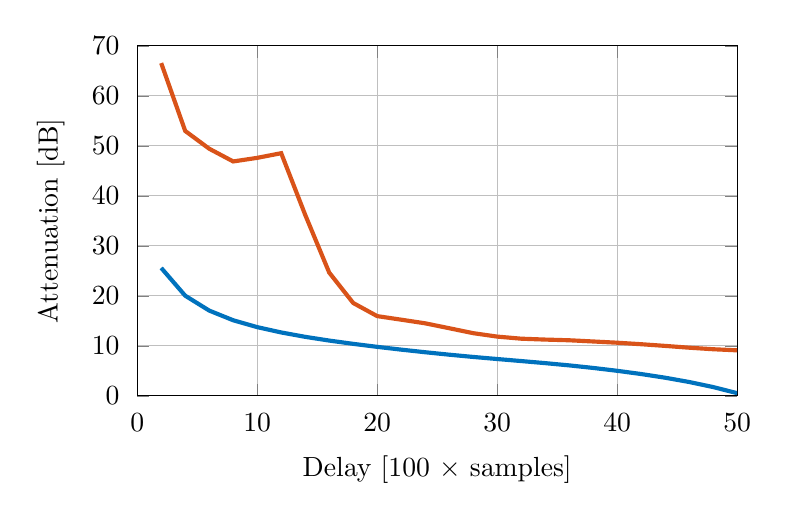
\begin{tikzpicture}

\begin{axis}[%
width=3in,
height=1.75in,
scale only axis,
xmin=0,
xmax=50,
xmajorgrids,
xlabel={Delay [100 $\times$ samples]},
ymin=0,
ymax=70,
ylabel style={yshift=0.3em},
xlabel style={yshift=-0.2em},
ytick={0,10,...,70},
ymajorgrids,
ylabel={Attenuation [dB]},
xticklabel shift={.1cm},
yticklabel shift={.1cm},
axis background/.style={fill=white}
]
\addplot [color=mycolor2,solid,line width=1.5pt,forget plot]
  table[row sep=crcr]{%
2	66.5420250310586\\
4	52.9717264302022\\
6	49.4175149424998\\
8	46.8717703569681\\
10	47.5886347675082\\
12	48.5221420089092\\
14	36.1913078215459\\
16	24.6480360536532\\
18	18.5625963047043\\
20	15.9345988709594\\
22	15.2225924490026\\
24	14.4941735350858\\
26	13.5145912190769\\
28	12.5242379572864\\
30	11.8400523957144\\
32	11.4203165228037\\
34	11.2428861871564\\
36	11.1050592495872\\
38	10.862823901561\\
40	10.6158645117455\\
42	10.3154480278615\\
44	9.97867799972119\\
46	9.61958031033587\\
48	9.31052791122033\\
50	9.08997582022533\\
};
\addplot [color=mycolor1,line width=1.5pt,solid,forget plot]
table[row sep=crcr]{%
	2	25.5751628128288\\
	4	20.0199680852144\\
	6	17.0442763613153\\
	8	15.1060127156582\\
	10	13.7310612019933\\
	12	12.6685774343164\\
	14	11.7903474171974\\
	16	11.0441690144364\\
	18	10.3883064900616\\
	20	9.78797702825996\\
	22	9.23075404560805\\
	24	8.7110676592604\\
	26	8.22176906503967\\
	28	7.77006791263877\\
	30	7.35426684398216\\
	32	6.94907270624338\\
	34	6.5323972441528\\
	36	6.08060777493347\\
	38	5.57101511941803\\
	40	4.99733350616245\\
	42	4.35167702165293\\
	44	3.61433096515684\\
	46	2.757705271237\\
	48	1.74470077738877\\
	50	0.5254168140125\\
};
\end{axis}
\end{tikzpicture}%
	\caption{Attenuation of feedforward FXLMS with different system delays.}
	\label{Fig:delayRatioAppendix}
\end{figure}

\subsection{Conclusion}
In a simulated real world infinite attenuation can be achieved if no delays are introduced. If simulated delays from sampling and reconstructing are introduced, the attenuation of the ANC system decrease.